\documentclass[10pt]{article}

\usepackage{sdss2020} % Uses Times Roman font (either newtx or times package)
\usepackage{url}
\usepackage{latexsym}
\usepackage{amsmath, amsthm, amsfonts}
\usepackage{algorithm, algorithmic}  
\usepackage{graphicx}

\usepackage[dvipsnames]{xcolor} % colors
\newcommand{\ear}[1]{{\textcolor{blue}{#1}}}
\newcommand{\svp}[1]{{\textcolor{RedOrange}{#1}}}
\newcommand{\rh}[1]{{\textcolor{Green}{#1}}}
\usepackage[capitalise]{cleveref}
\newcommand\pcref[1]{(\cref{#1})}

\title{`You Draw It': Implementation of visually fitted trends with
\texttt{r2d3}}

%\author{by }
\author{
  Emily A. Robinson \\
  \small{University of Nebraska - Lincoln}\\
  \small{Lincoln, NE} \\
  \small{\tt emily.robinson@huskers.unl.edu} \\\And
 Reka Howard \\
  \small{University of Nebraska - Lincoln}\\
  \small{Lincoln, NE} \\
  \small{\tt rekahoward@unl.edu} \\\And
  Susan VanderPlas \\
  \small{University of Nebraska - Lincoln}\\
  \small{Lincoln, NE} \\
  \small{\tt susan.vanderplas@unl.edu} \\}

\date{}

\begin{document}
\maketitle
\begin{abstract}
How do statistical regression results compare to intuitive, visually
fitted results? Fitting lines by eye through a set of points has been
explored since the 20th century. Common methods of fitting trends by eye
involve maneuvering a string, black thread, or ruler until the fit is
suitable, then drawing the line through the set of points. In 2015, the
New York Times introduced an interactive feature, called `You Draw It,'
where readers are asked to input their own assumptions about various
metrics and compare how these assumptions relate to reality. This
research is intended to implement `You Draw It', adapted from the New
York Times, as a way to measure the patterns we see in data.
\end{abstract}

{\bf Keywords:} graphics, user interaction, regression

\section{Introduction}

We all use statistical graphics, but how do we know that the graphics we
use are communicating {\textcolor{RedOrange}{effectively}}? Through
experimentation, graphical testing methods allow researchers to conduct
studies
{\textcolor{RedOrange}{designed to understand how we perceive graphics and perform graphical tasks}}
such as differentiation, prediction, estimation, and extrapolation.
{\textcolor{RedOrange}{Each of these levels of interaction with a graph require a different method of engagement with and use of the information presented in a chart.}}
{\textcolor{RedOrange}{In this paper, we describe the adaptation of an old tool for graphical testing and evaluation, eye-fitting, for use in modern web-applications suitable for testing statistical graphics. 
We present an empirical evaluation of this testing method for linear regression, and briefly discuss an extension of this method to non-linear applications.}}

\subsection{Measuring Patterns and Trends}

{\textcolor{RedOrange}{One of the most common charts created is a scatter plot of points over time; these charts show up regularly in news articles and in scientific publications alike.
These charts rely on our}} ability to identify and detect trends in
data. Our visual system is naturally built to look for structure and
identify patterns,
{\textcolor{RedOrange}{including patterns and trends over time; many times we do not even notice this process happening subconsciously}}.
{\textcolor{RedOrange}{As shown in \cref{fig:gas-prices}, a viewer engaging with a plot of weekly average gas prices over time may perform several cognitive operations. First, they scan the plot and assesses points to determine if there are any outliers or otherwise remarkable points. Then, they may fit a rough mental smooth/trend line to the points to summarize the useful information and remove variability. Finally, an interested and engaged viewer may pull in additional contextual information from long-term memory, seeking to explain variation in the mental 'trend' with supplemental information, such as COVID lock downs which reduced gasoline demand and the beginning of the war in Ukraine, which wreaked havoc on the supply and demand for global energy sources.}}

\begin{figure}

{\centering 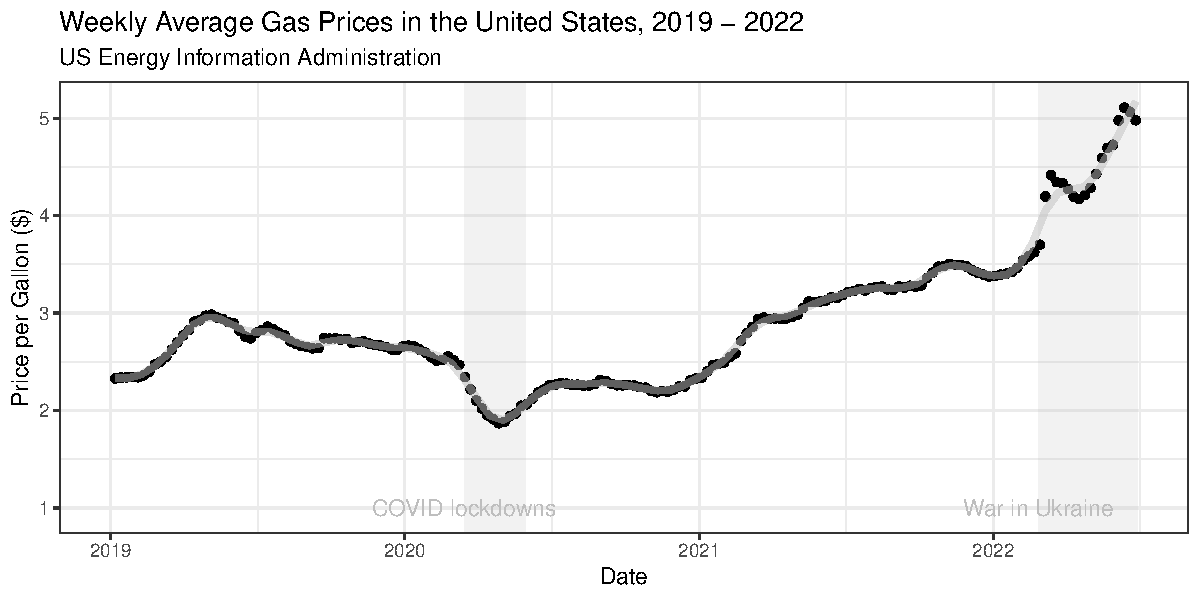
\includegraphics[width=\columnwidth]{./images/gas-prices-1} 

}

\caption{Weekly average gas prices in the United States, 2019-June 2022. Additional mental operations a viewer might perform while looking at the plot are annotated in grey. \cite{usenergyinformationadministrationWeeklyAllGrades2022}.}\label{fig:gas-prices}
\end{figure}

Initial studies in the 20th century explored the use of fitting lines by
eye through a set of points
\cite{finney1951subjective,mosteller1981eye}. Common methods of fitting
trends by eye involved maneuvering a string, black thread, or ruler
until the fit was suitable, then drawing the line through the set of
points. Recently, Ciccione and Dehaene \shortcite{ciccione2021can}
conducted a comprehensive set of studies investigating human ability to
detect trends in graphical representations from a psychophysical
approach.{\textcolor{RedOrange}{XXX and found what? Describe the results XXX}}

{\textcolor{RedOrange}{While psychologists and statisticians have been using eye-fitting techniques to assess our innate perceptual statistical modeling abilities, news organizations have used similar techniques in order to draw readers in and demonstrate the difference between readers' assumptions and reality.}}
In 2015, the New York Times introduced an interactive feature, called
`You Draw It' \cite{aisch2015you}, where readers input their own
assumptions about various
{\textcolor{RedOrange}{metrics of news interest}} and compare these
assumptions to reality. The New York Times team used Data Driven
Documents (D3), {\textcolor{RedOrange}{a JavaScript library}} that
allows readers to
{\textcolor{RedOrange}{interact with a chart directly by}} drawing a
line on their computer screen with a mouse.
{\textcolor{RedOrange}{Despite the somewhat different purpose behind this feature, the D3 driven method used by the NYT is wonderfully intuitive, and does not require the assumption of linearity, making it much more adaptable to testing how viewers perceive and predict when presented with non-linear data.}}

{\textcolor{RedOrange}{We set out to implement}} `You Draw It', adapted
from the New York Times feature, as a way to measure the patterns we see
in data. Here, we provide technical details of the software development,
utilizing interactive graphics in R\cite{r-software}. We then share
results from our study which validates `You Draw It' as a method for
graphical testing {\textcolor{RedOrange}{on linear trends}} and apply an
appropriate data analysis method to the participant data.
{\textcolor{RedOrange}{We also briefly demonstrate the use of the 'You Draw It' method and analysis on nonlinear data.}}

\section{Development}

\subsection{`You Draw It' Task}

When completing the graphical task, users are shown an interactive
scatter-plot (Figure 1) along with the prompt, ``Use your mouse to fill
in the trend in the yellow box region.'' The yellow box region moves
along as the user draws their trend-line, providing a visual cue which
indicates where the user still needs to complete a trend line. After the
entire domain has been visually estimated or predicted, the yellow
region disappears, indicating the participant has completed the task.
Prior to study participation, example gifs are shown and users are asked
to complete practice plots to ease the learning curve of the task.
\footnote{Visit \url{emily-robinson.shinyapps.io/can-you-draw-it} for a
  test applet.}

\begin{figure}[ht]
\begin{center}
\centerline{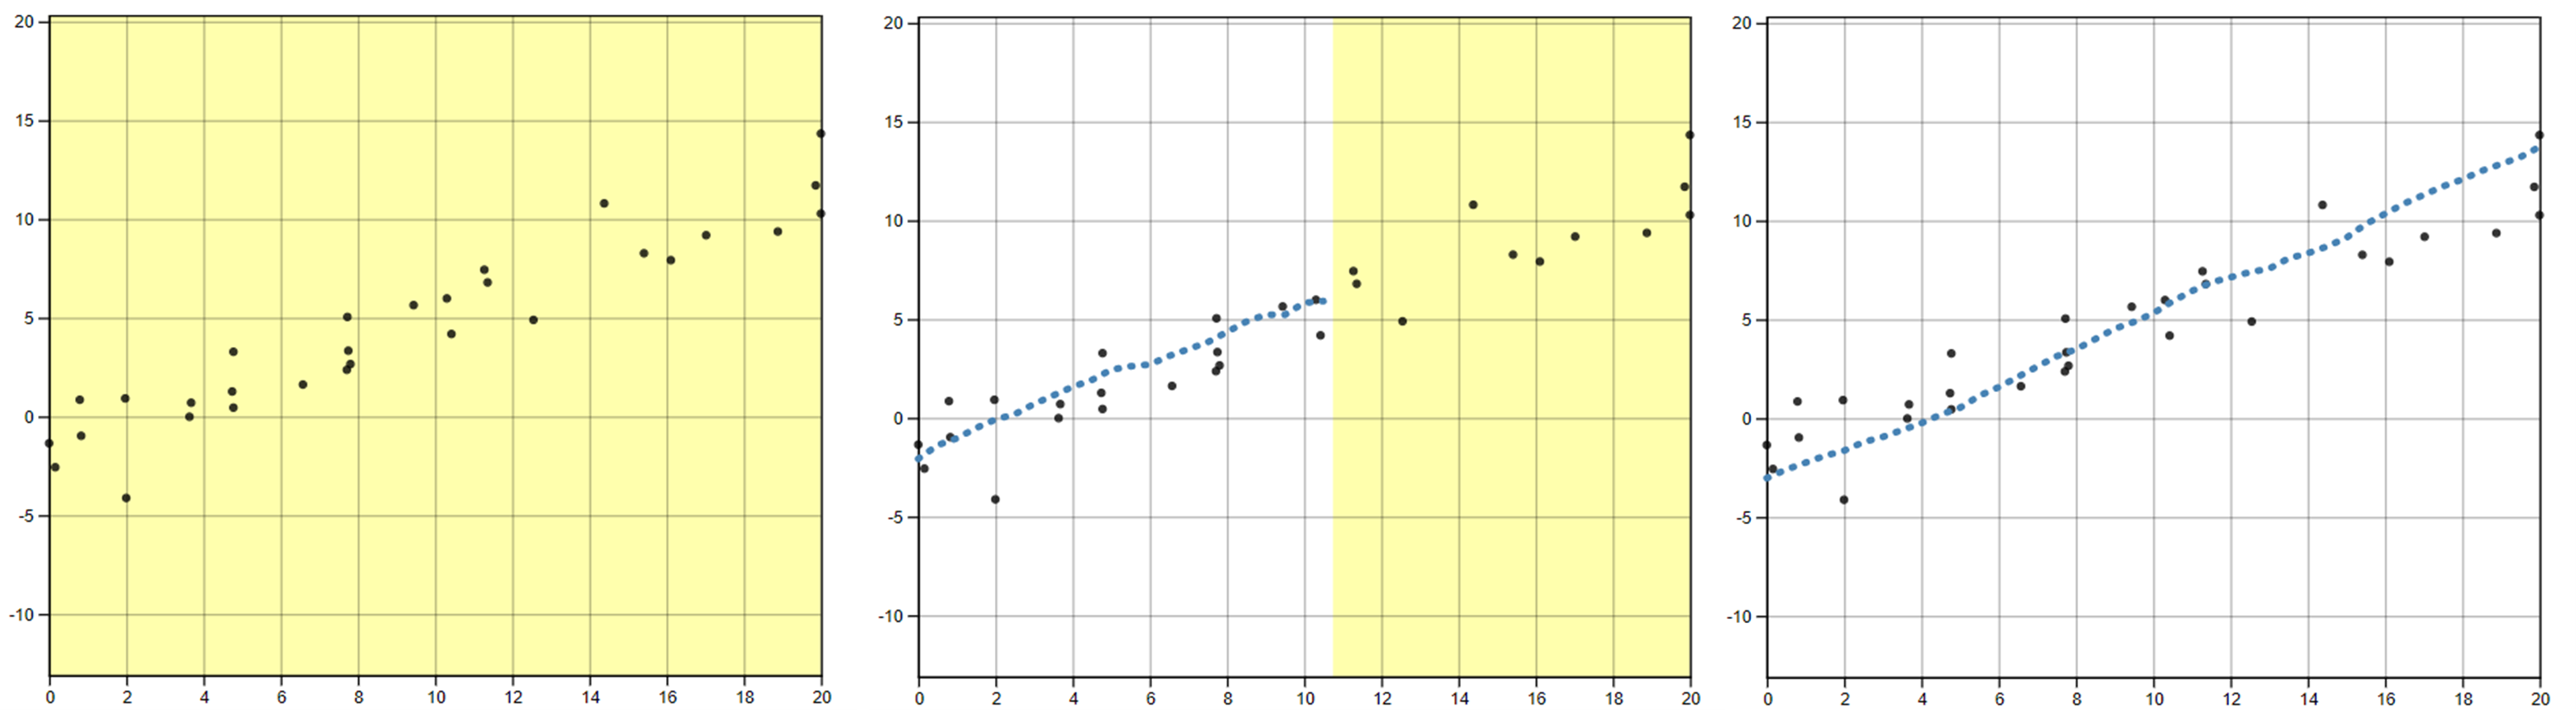
\includegraphics[width=\columnwidth]{images/ydi-stimuli}}
\caption{You Draw It' task plot as shown to user. \\
\textbf{left:} illustrates what user first sees with the prompt \textit{Use your mouse to fill in the trend in the yellow box region.} \\
\textbf{middle:} illustrates what the user sees while completing the task.\\
\textbf{right:} illustrates the users finished trend line.}
\label{you-draw-it-task-plot}
\end{center}
\end{figure}

\subsection{Code Sketch}

Using Shiny \cite{shinypkg} and JavaScript, we modified the New York
Times `You Draw It' feature for the purpose of testing statistical
graphics allowing us to incorporate user interaction, conduct studies
online, and store participant responses.

Data Driven Documents (D3) \cite{bostock2011d3}, a JavaScript-based
graphing framework that facilitates user interaction, was used to create
the `You Draw It' visual. Major news and research organizations such as
the New York Times, FiveThirtyEight, Washington Post, and the pew
Research Center use D3 to create and customize graphics. A challenge of
working with D3 is the environment necessary to display the graphics and
images. The \texttt{r2d3} package \cite{r2d3pkg} provides an efficient
integration of D3 visuals into R HTML formats. We integrate the D3
visual source code into an R Shiny \cite{shinypkg} application in order
to allow for user interaction and data collection.

Figure 2 illustrates the initial setup of the visual stimuli along with
the iterative process between the user interaction and plotting. We
conducted all data simulation and processing in R and output two data
sets - \emph{point data} and \emph{line data} - containing (x, y)
coordinates corresponding to either a simulated point or fitted value
predicted by a statistical model respectively. Then, the r2d3 package
converts the data sets in R to JavaScript Object Notation (JSON) to be
interpreted by the \texttt{D3.js} code. We define functions in
\texttt{D3.js} to draw the initial plot and set up drawable points for
the user drawn line. Drag events in \texttt{D3.js} are utilized to
observe and react to user input. Shiny Messages are used to communicate
the user interaction between the \texttt{D3.js} code and the R
environment. The plot is then rendered and updated on user interaction
into the R shiny application with the \texttt{RenderD3} and
\texttt{d3Output} functions. Once the user is done drawing the line, we
saved the results of the drawn line to a database for analysis.

\begin{figure}[ht]
\begin{center}
\centerline{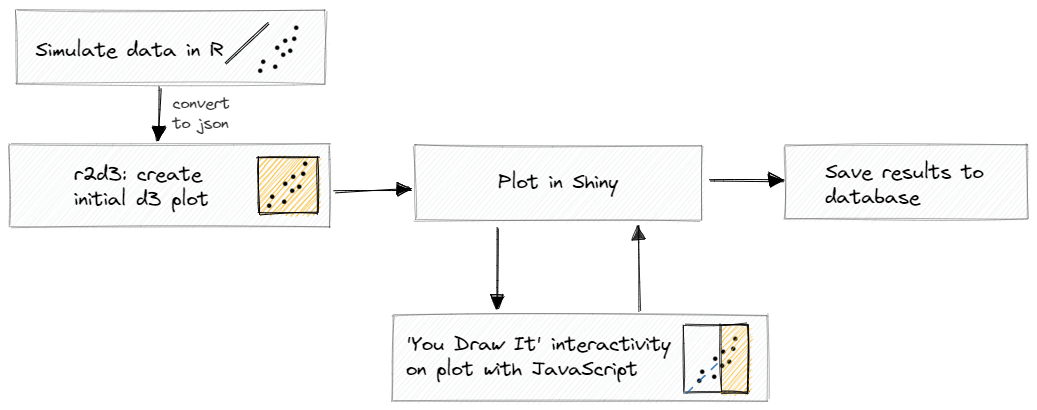
\includegraphics[width=\columnwidth]{images/code-sketch-2}}
\caption{Sketch of underlying code for 'You Draw It', illustrating the data simulation conducted in R, the initial setup of the visual stimuli with D3 source code, along with the iterative process between the user interaction and plotting in Shiny. Once the user is done drawing the line, we saved the results of the drawn line to a database for analysis.}
\label{you-draw-it-code-sketch}
\end{center}
\end{figure}

Parameters for aesthetic design choices are defined in a list of options
and \texttt{r2d3} passes these to the D3.js code. For instance, we can
specify the buffer space allowed for the \(x\) and \(y\) axes to avoid
users to anchor their lines to the axes limits. \footnote{For
  \texttt{D3.js} source code, visit
  \url{https://github.com/earobinson95/presentations/blob/master/can-you-draw-it/www/main-d3v5.js}.}

\subsection{Challenges}

During the development process, there were a few challenges we had to
overcome. We documented these challenges with GitHub commits and outline
places where frustration occurred. Data Driven documents uses Scalable
Vector Graphics (SVG), thus requiring careful transformation between the
pixels and plot coordinates to align the simulated data and the user
drawn line appropriately. With the layered framework of SVG's, it was
important to place the layers in the right order so certain features
would appear where desired. For example, we wanted the opacity of the
yellow box region to appear under the points while still showing the
grid lines. As previously mentioned, \texttt{r2d3} automatically
converts the data set to a JSON file to be interpreted by the underlying
source code, however we provided two data sets (point data and line
data) and converted the two data sets to a JSON file before passing them
to the \texttt{r2d3} argument so that we could reference both data sets
within the \texttt{D3.js} code. One constraint of the development code
to date is that it is only built to work with one-to-one functions and
does not allow for multiple estimates or predictions for one
\(x\)-value.

\section{Application}

\subsection{Tool Validation}

We conducted a study in order to validate `You Draw It' as a method for
graphical testing, comparing results to the less technological method
utilized in Mosteller et al.~\shortcite{mosteller1981eye}. Results from
our study were consistent with those found in the previous study; when
shown points following a linear trend, participants tended to fit the
slope of the first principal component over the slope of the ordinary
least-squares regression line (Figure 3). This trend was most prominent
when shown data simulated with larger variances. This study reinforced
the differences between intuitive visual model fitting and statistical
model fitting, providing information about human perception as it
relates to the use of statistical graphics.

\begin{figure}[ht]
\begin{center}
\centerline{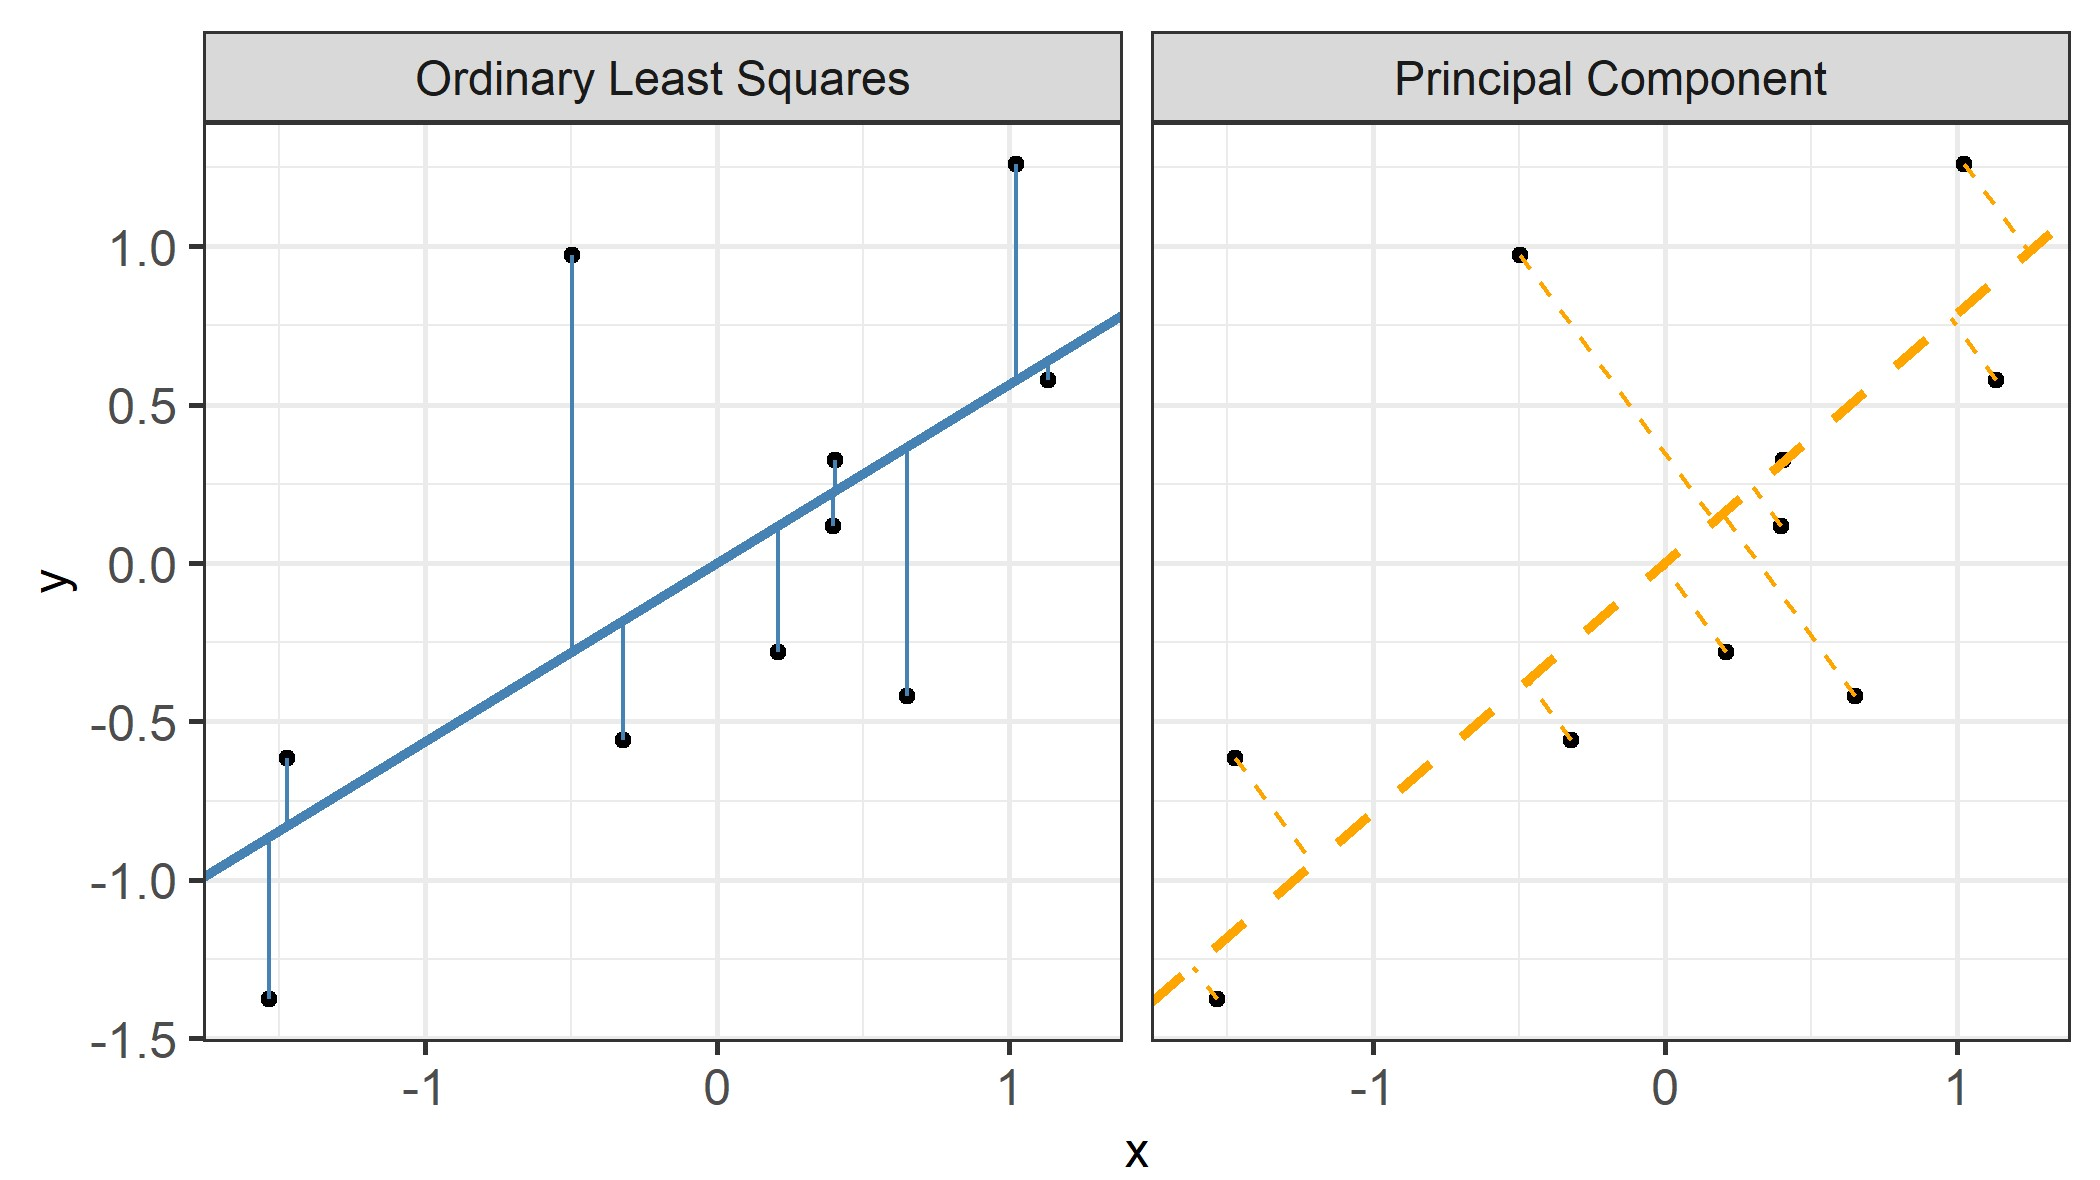
\includegraphics[width=\columnwidth]{images/pca-plot}}
\caption{Comparison between an OLS regression equation which minimizes the vertical distance of points from the line and a regression equation with a slope calculated by the first principal component which minimizes the smallest distance of points from the line.}
\label{pca-plot}
\end{center}
\end{figure}

\subsection{Data Analysis}

\begin{figure}[ht]
\begin{center}
\centerline{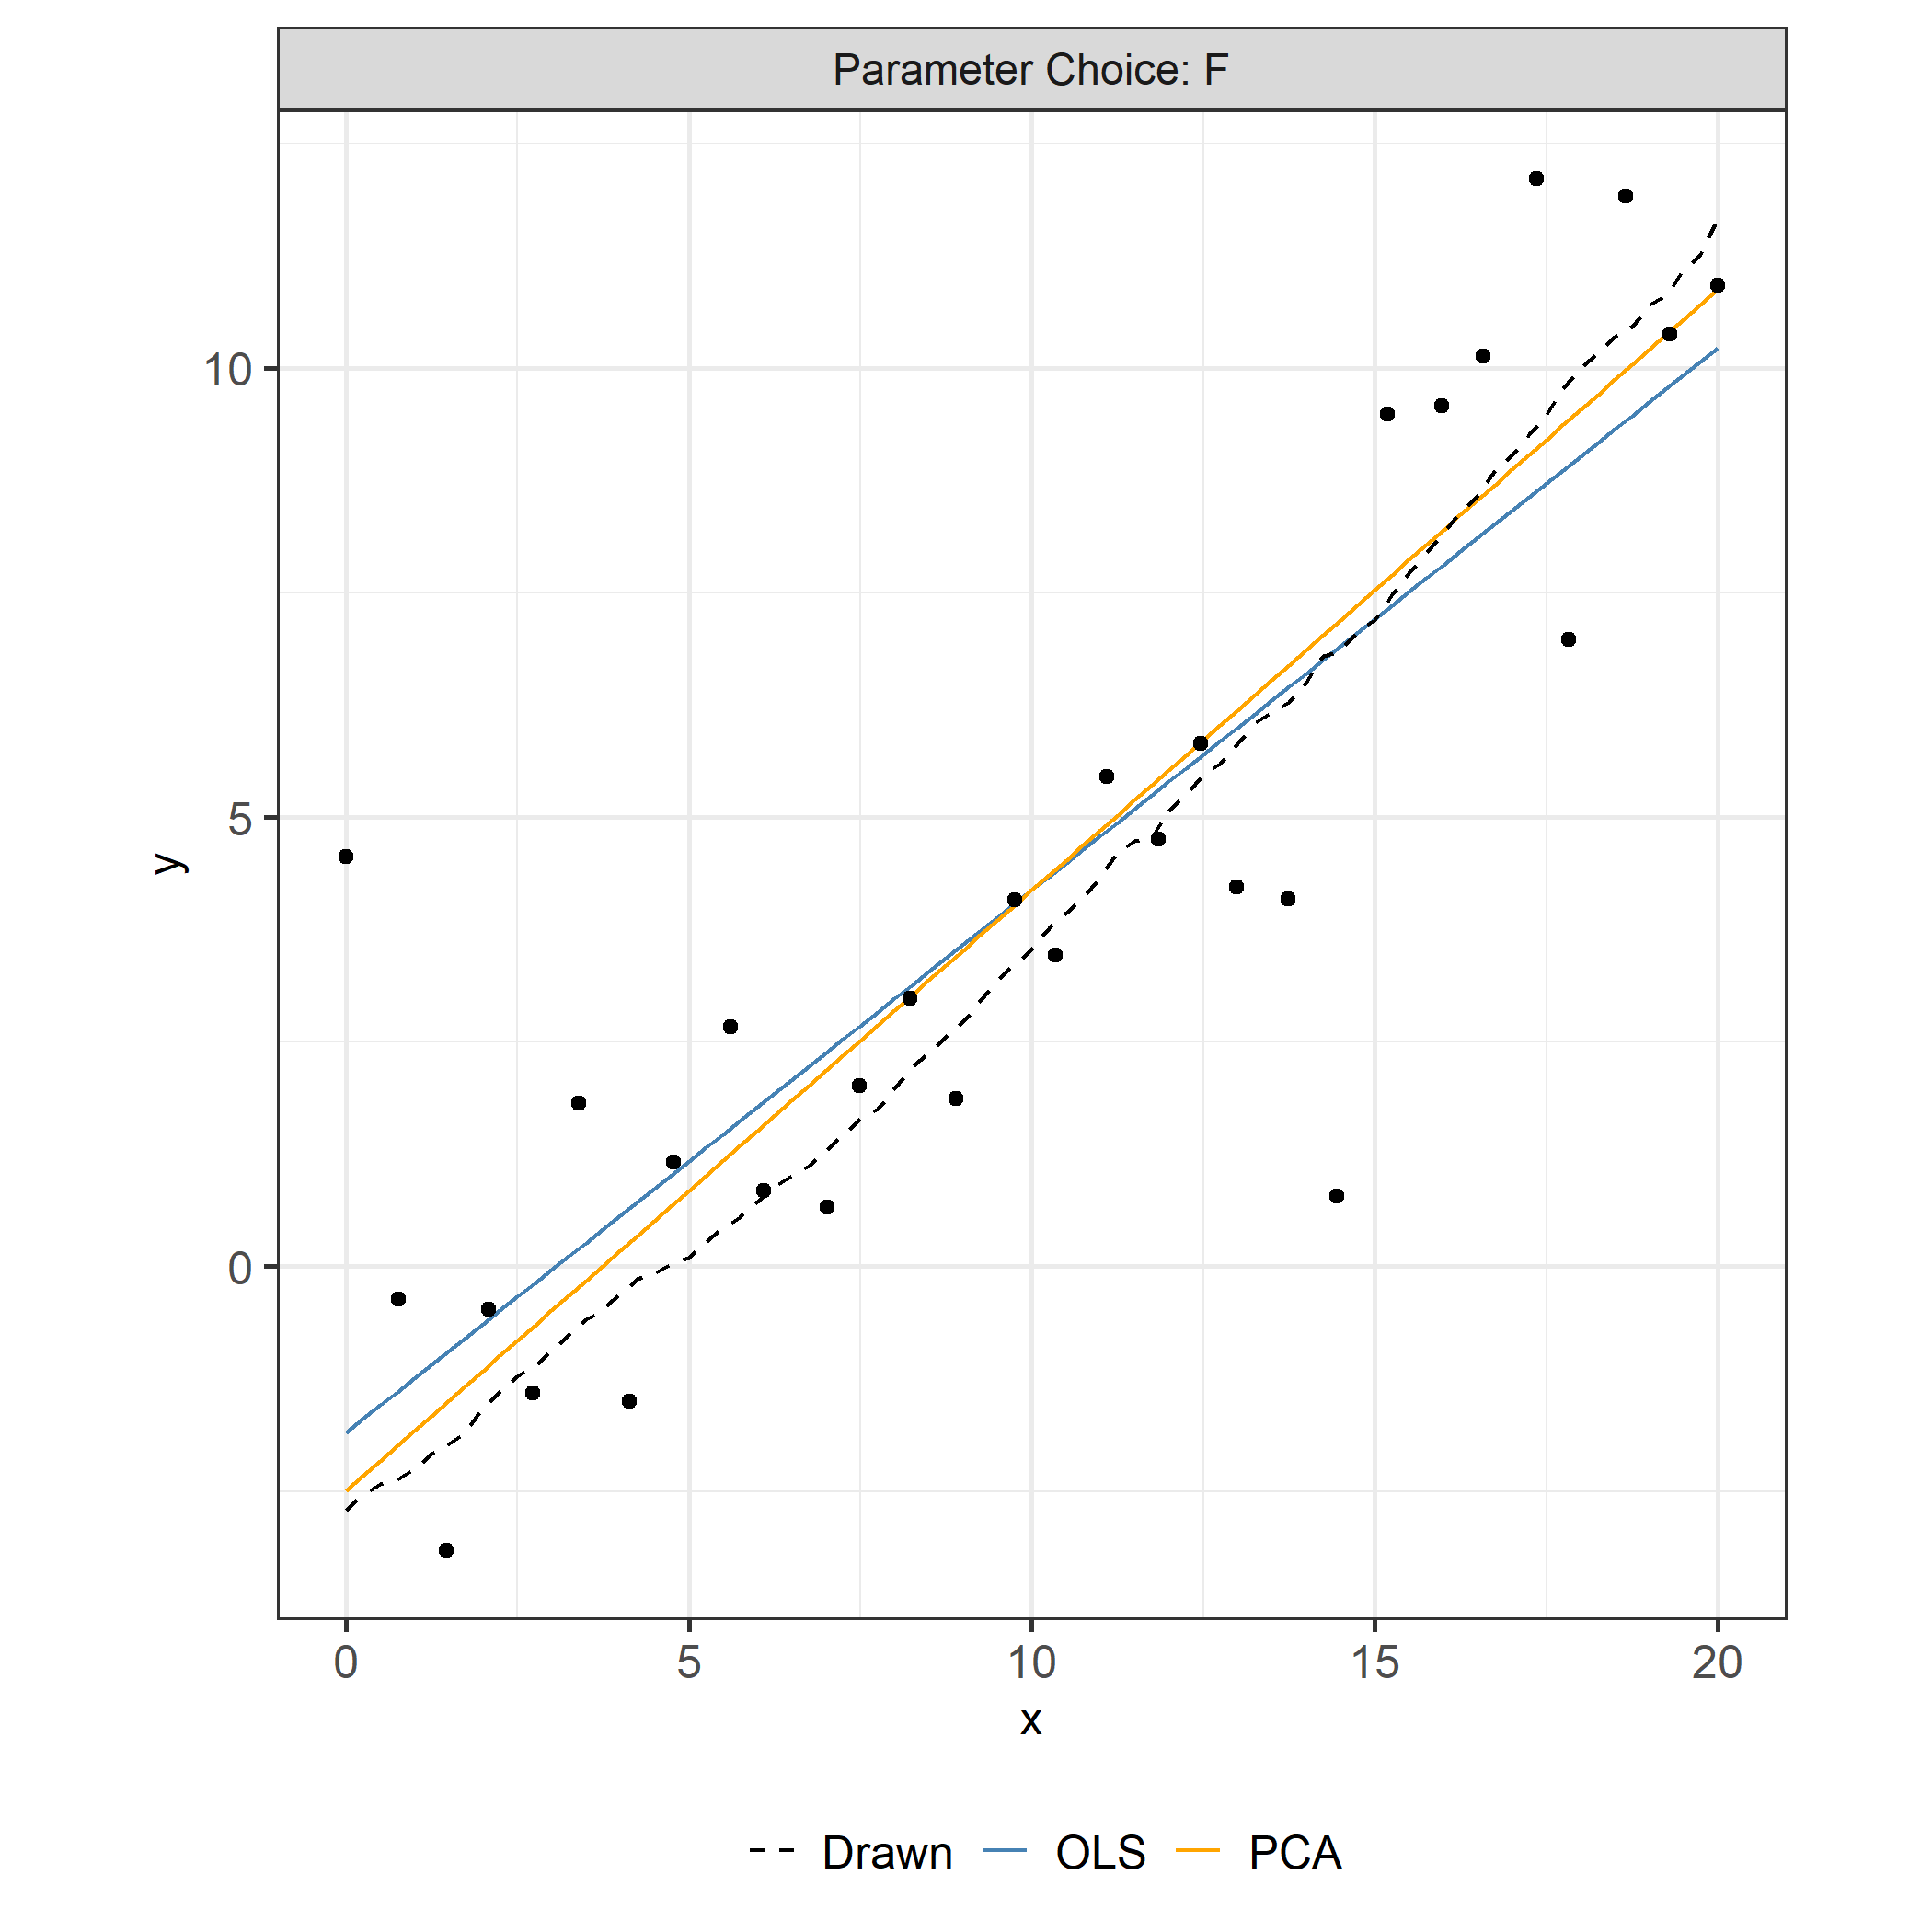
\includegraphics[width=\columnwidth]{images/eyefitting-trial-plot}}
\caption{Example of validation feedback data where three trend lines show the the OLS fitted, PCA fitted, and participant drawn values overlaid on the simulated data points}
\label{eyefitting-trial-plot}
\end{center}
\end{figure}

Feedback data from conducted studies were collected and stored in a
database for analysis (Figure 4). Within the collected feedback data, we
knew the simulated data points, the predicted values from the
statistical model, and the predicted values from the user drawn line. In
our initial studies, a unique data set was simulated independently for
each participant. Therefore, we evaluate the accuracy of the user drawn
line by observing the deviation, vertical residuals, between the user
drawn line and the predicted values from the statistical model. Due to
participant variation, we use mixed models to evaluate the vertical
residuals in order to statistically compare visually fitted trends to
actual metrics, simulated data models, or statistical regression
results. In our validation study, we first analyzed the residual trend
using a linear mixed model (LMM), thus constraining the fit to a linear
trend (Figure 5). In addition, we fit a Generalized Additive Mixed Model
(GAMM) to allow for flexibility in the residual trend and to generalized
the method to nonlinear models (Figure 6).

\begin{figure}[ht]
\begin{center}
\centerline{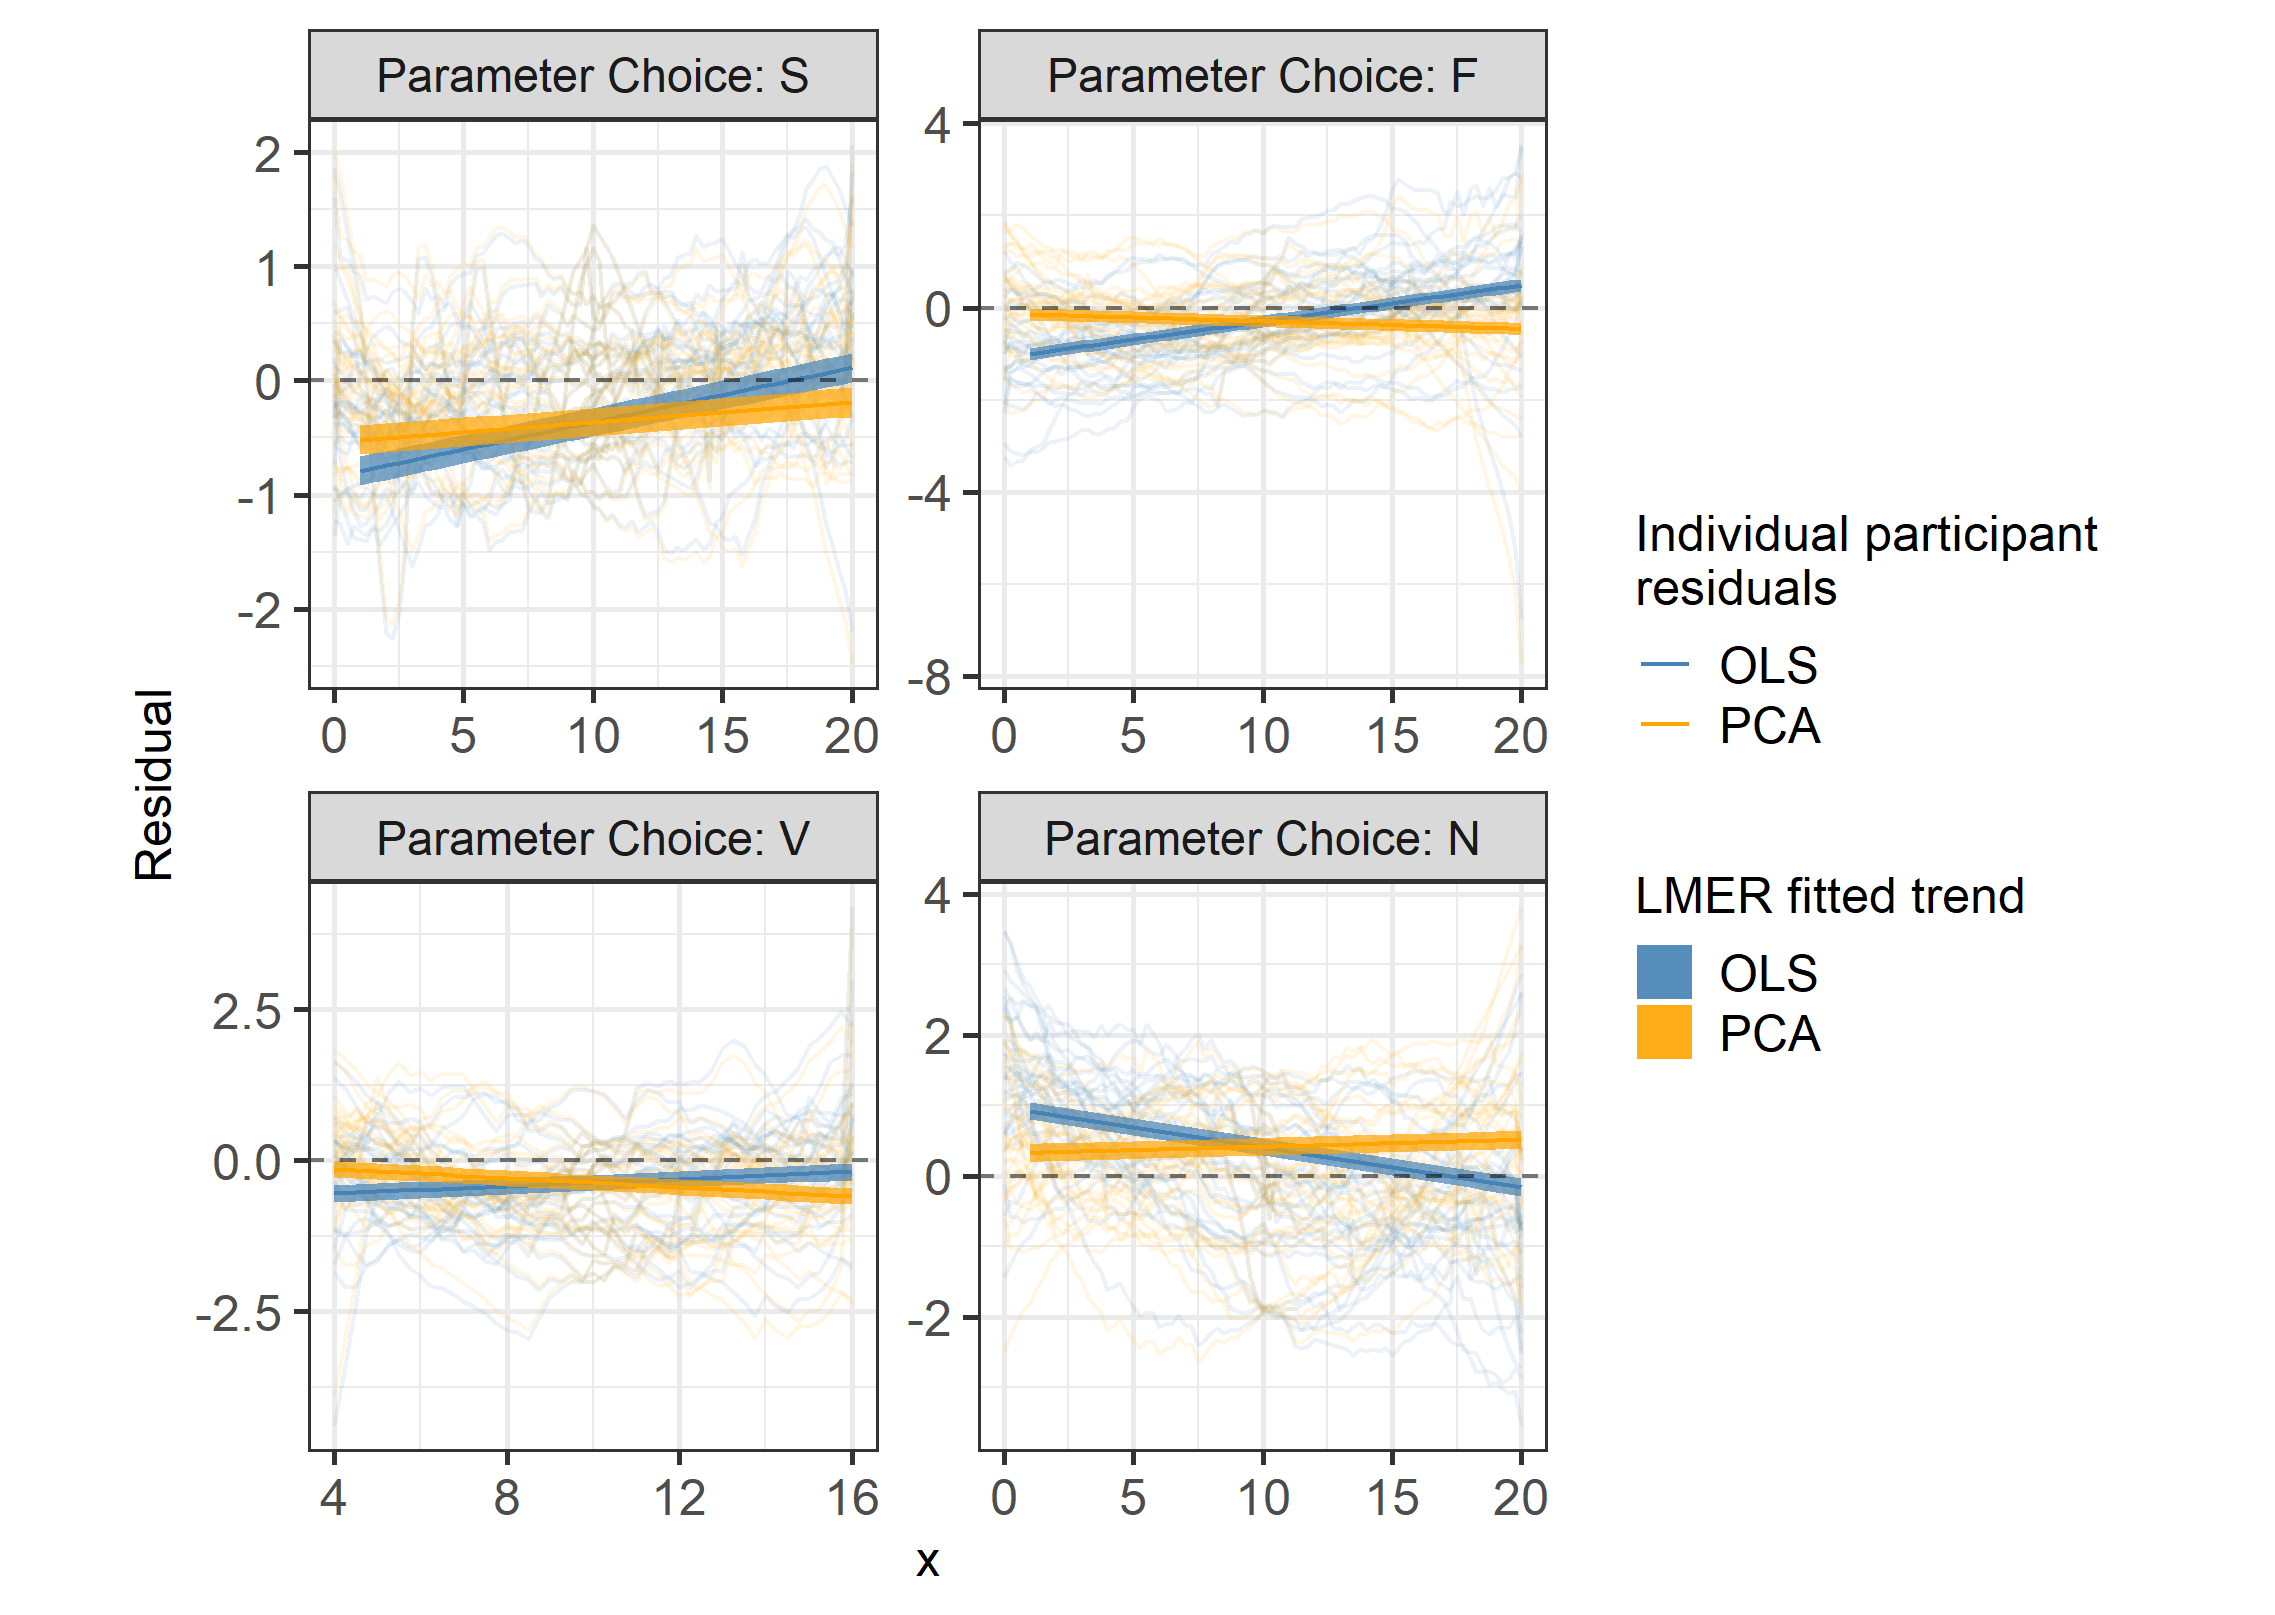
\includegraphics[width=\columnwidth]{images/eyefitting-lmer-plot}}
\caption{Validation study estimated trends of residuals (vertical deviation of participant drawn points from both the OLS (blue) and PCA (orange) fitted points) as fit by a linear mixed model.}
\label{eyefitting-lmer-plot}
\end{center}
\end{figure}

\begin{figure}[ht]
\begin{center}
\centerline{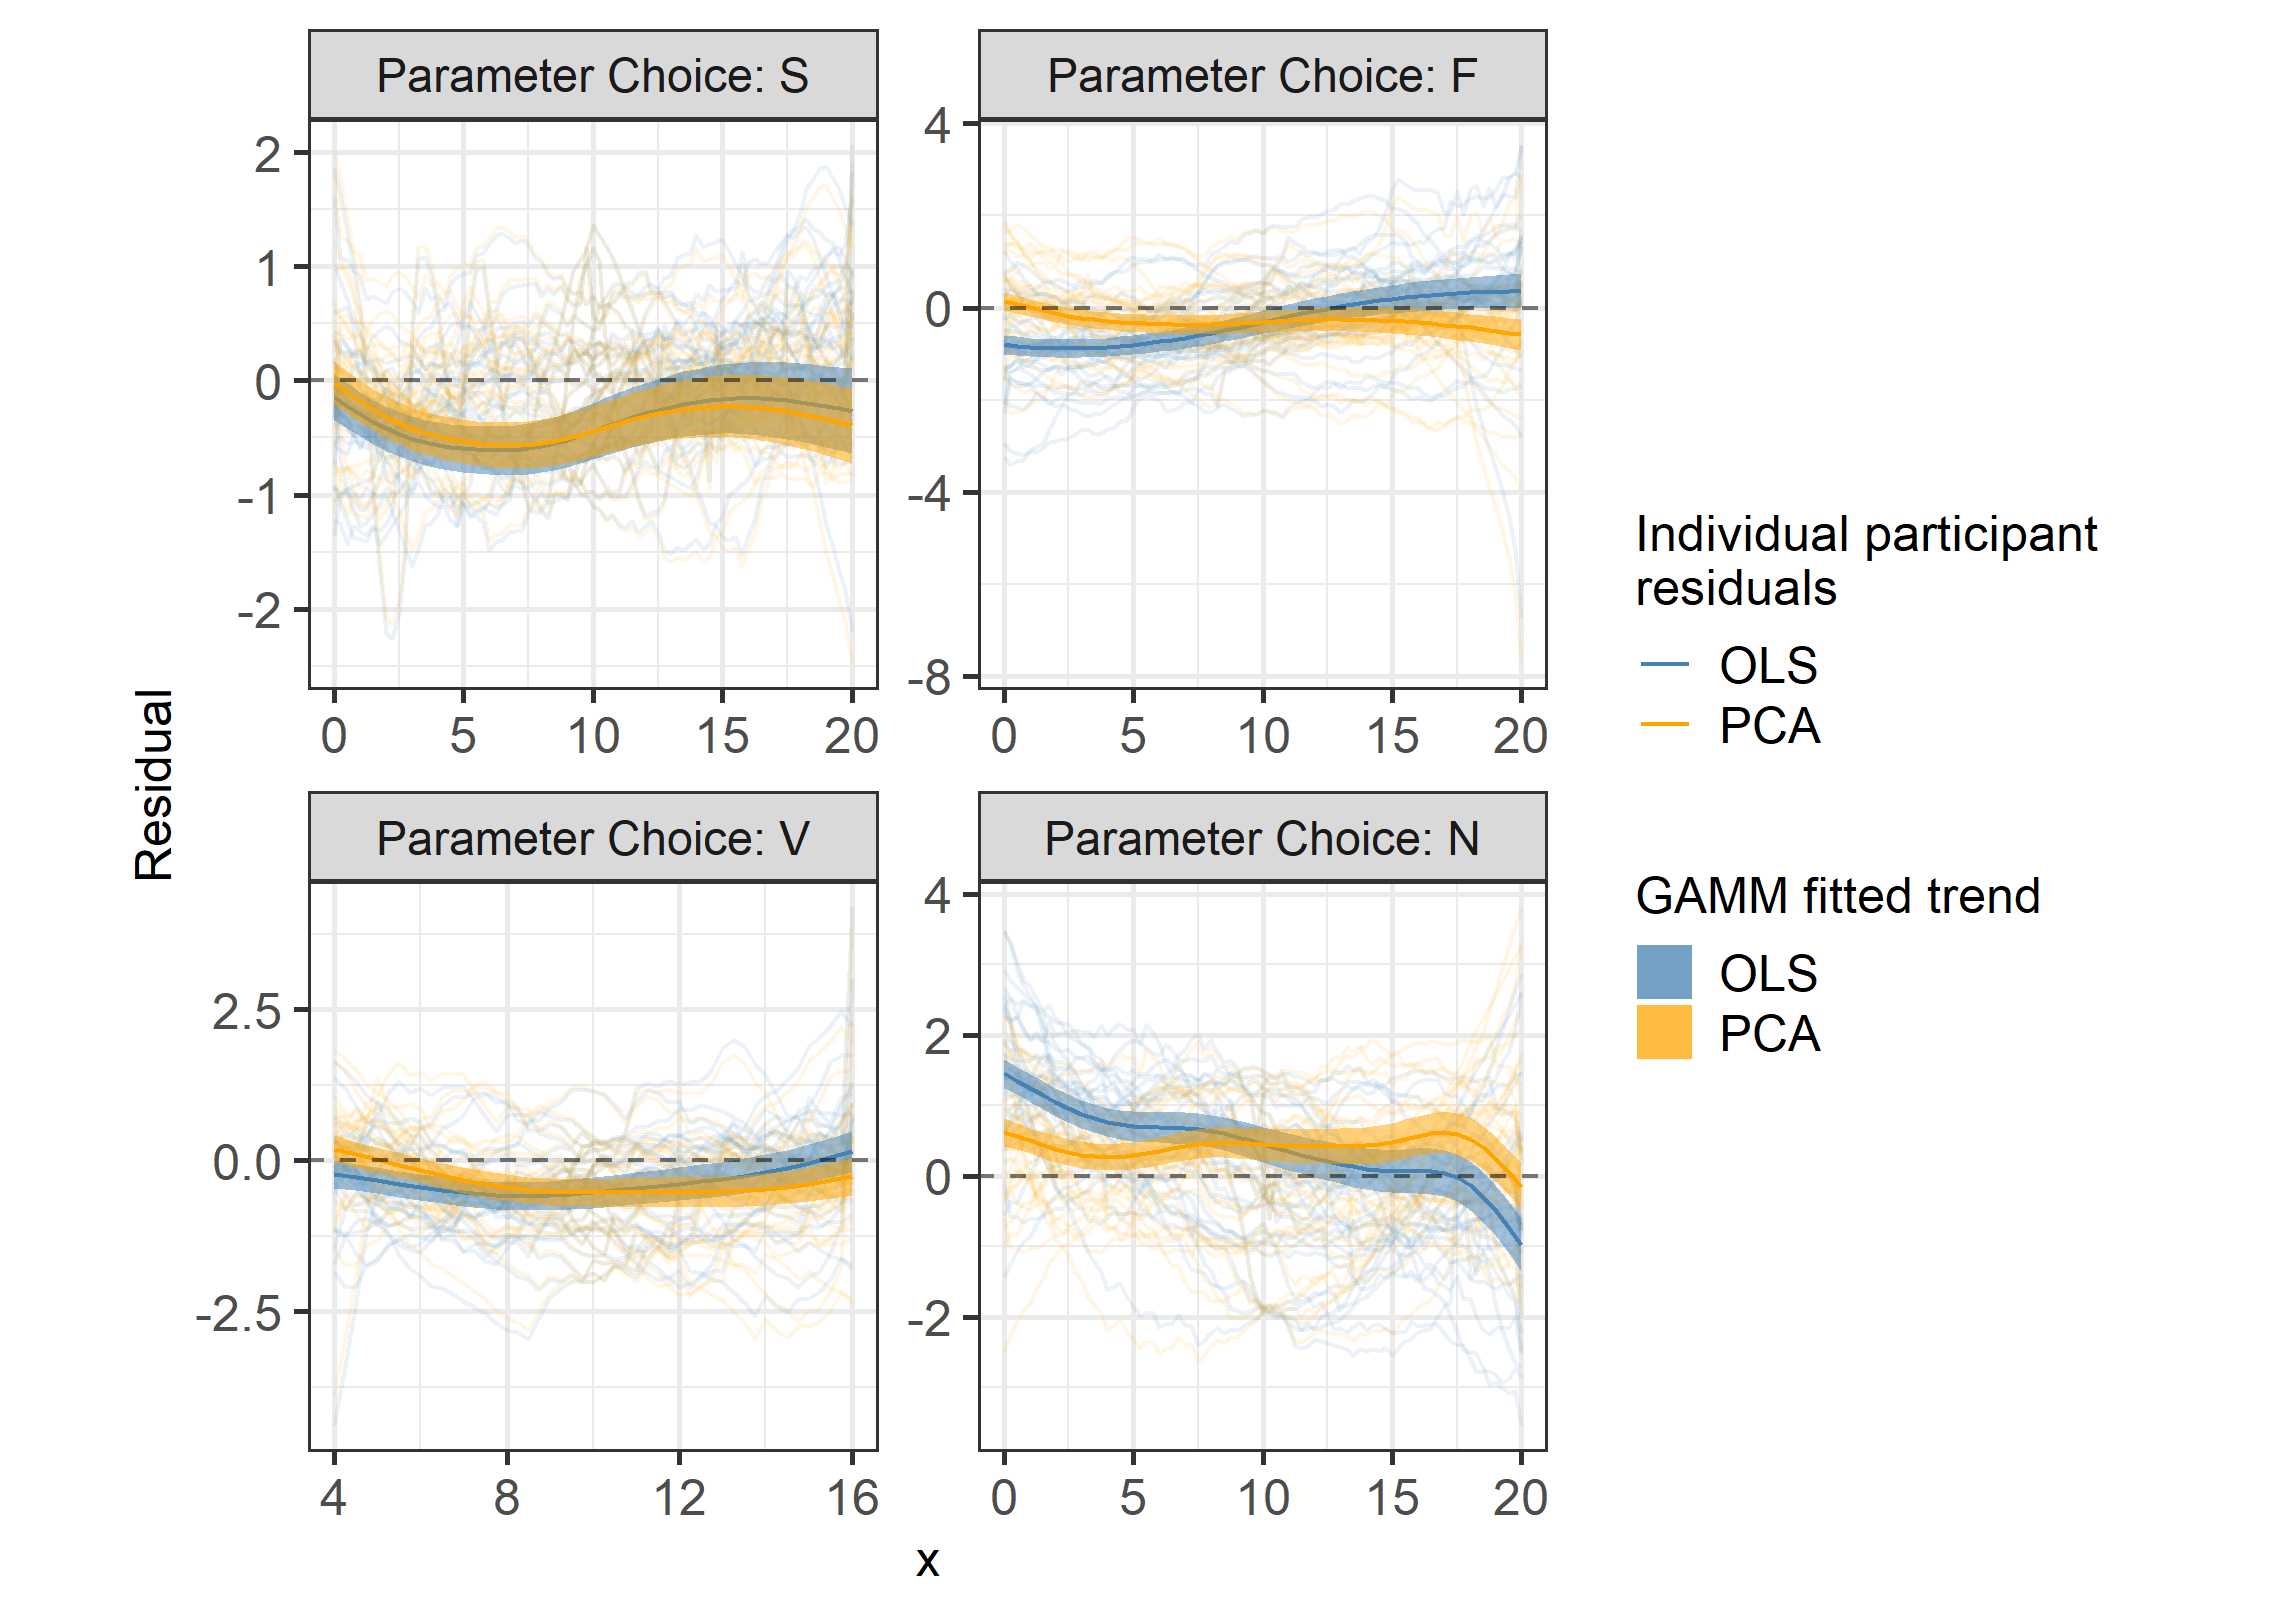
\includegraphics[width=\columnwidth]{images/eyefitting-gamm-plot}}
\caption{Validation study estimated trends of residuals (vertical deviation of participant drawn points from both the OLS (blue) and PCA (orange) fitted points) as fit by a generalized additive mixed model.}
\label{eyefitting-gamm-plot}
\end{center}
\end{figure}

After validating the `You Draw It' method, we conducted a study
utilizing the new method to evaluate participants ability to make
forecasts for exponentially increasing data on log and linear scales.
Along with analyzing the feedback data with the GAMM method for
flexibility due to nonlinear data, we used spaghetti plots to visualize
participants forecasts compared to the nonlinear least squares
statistical model and make comparisons between two chart design features
(Figure 6).

\begin{figure}[ht]
\begin{center}
\centerline{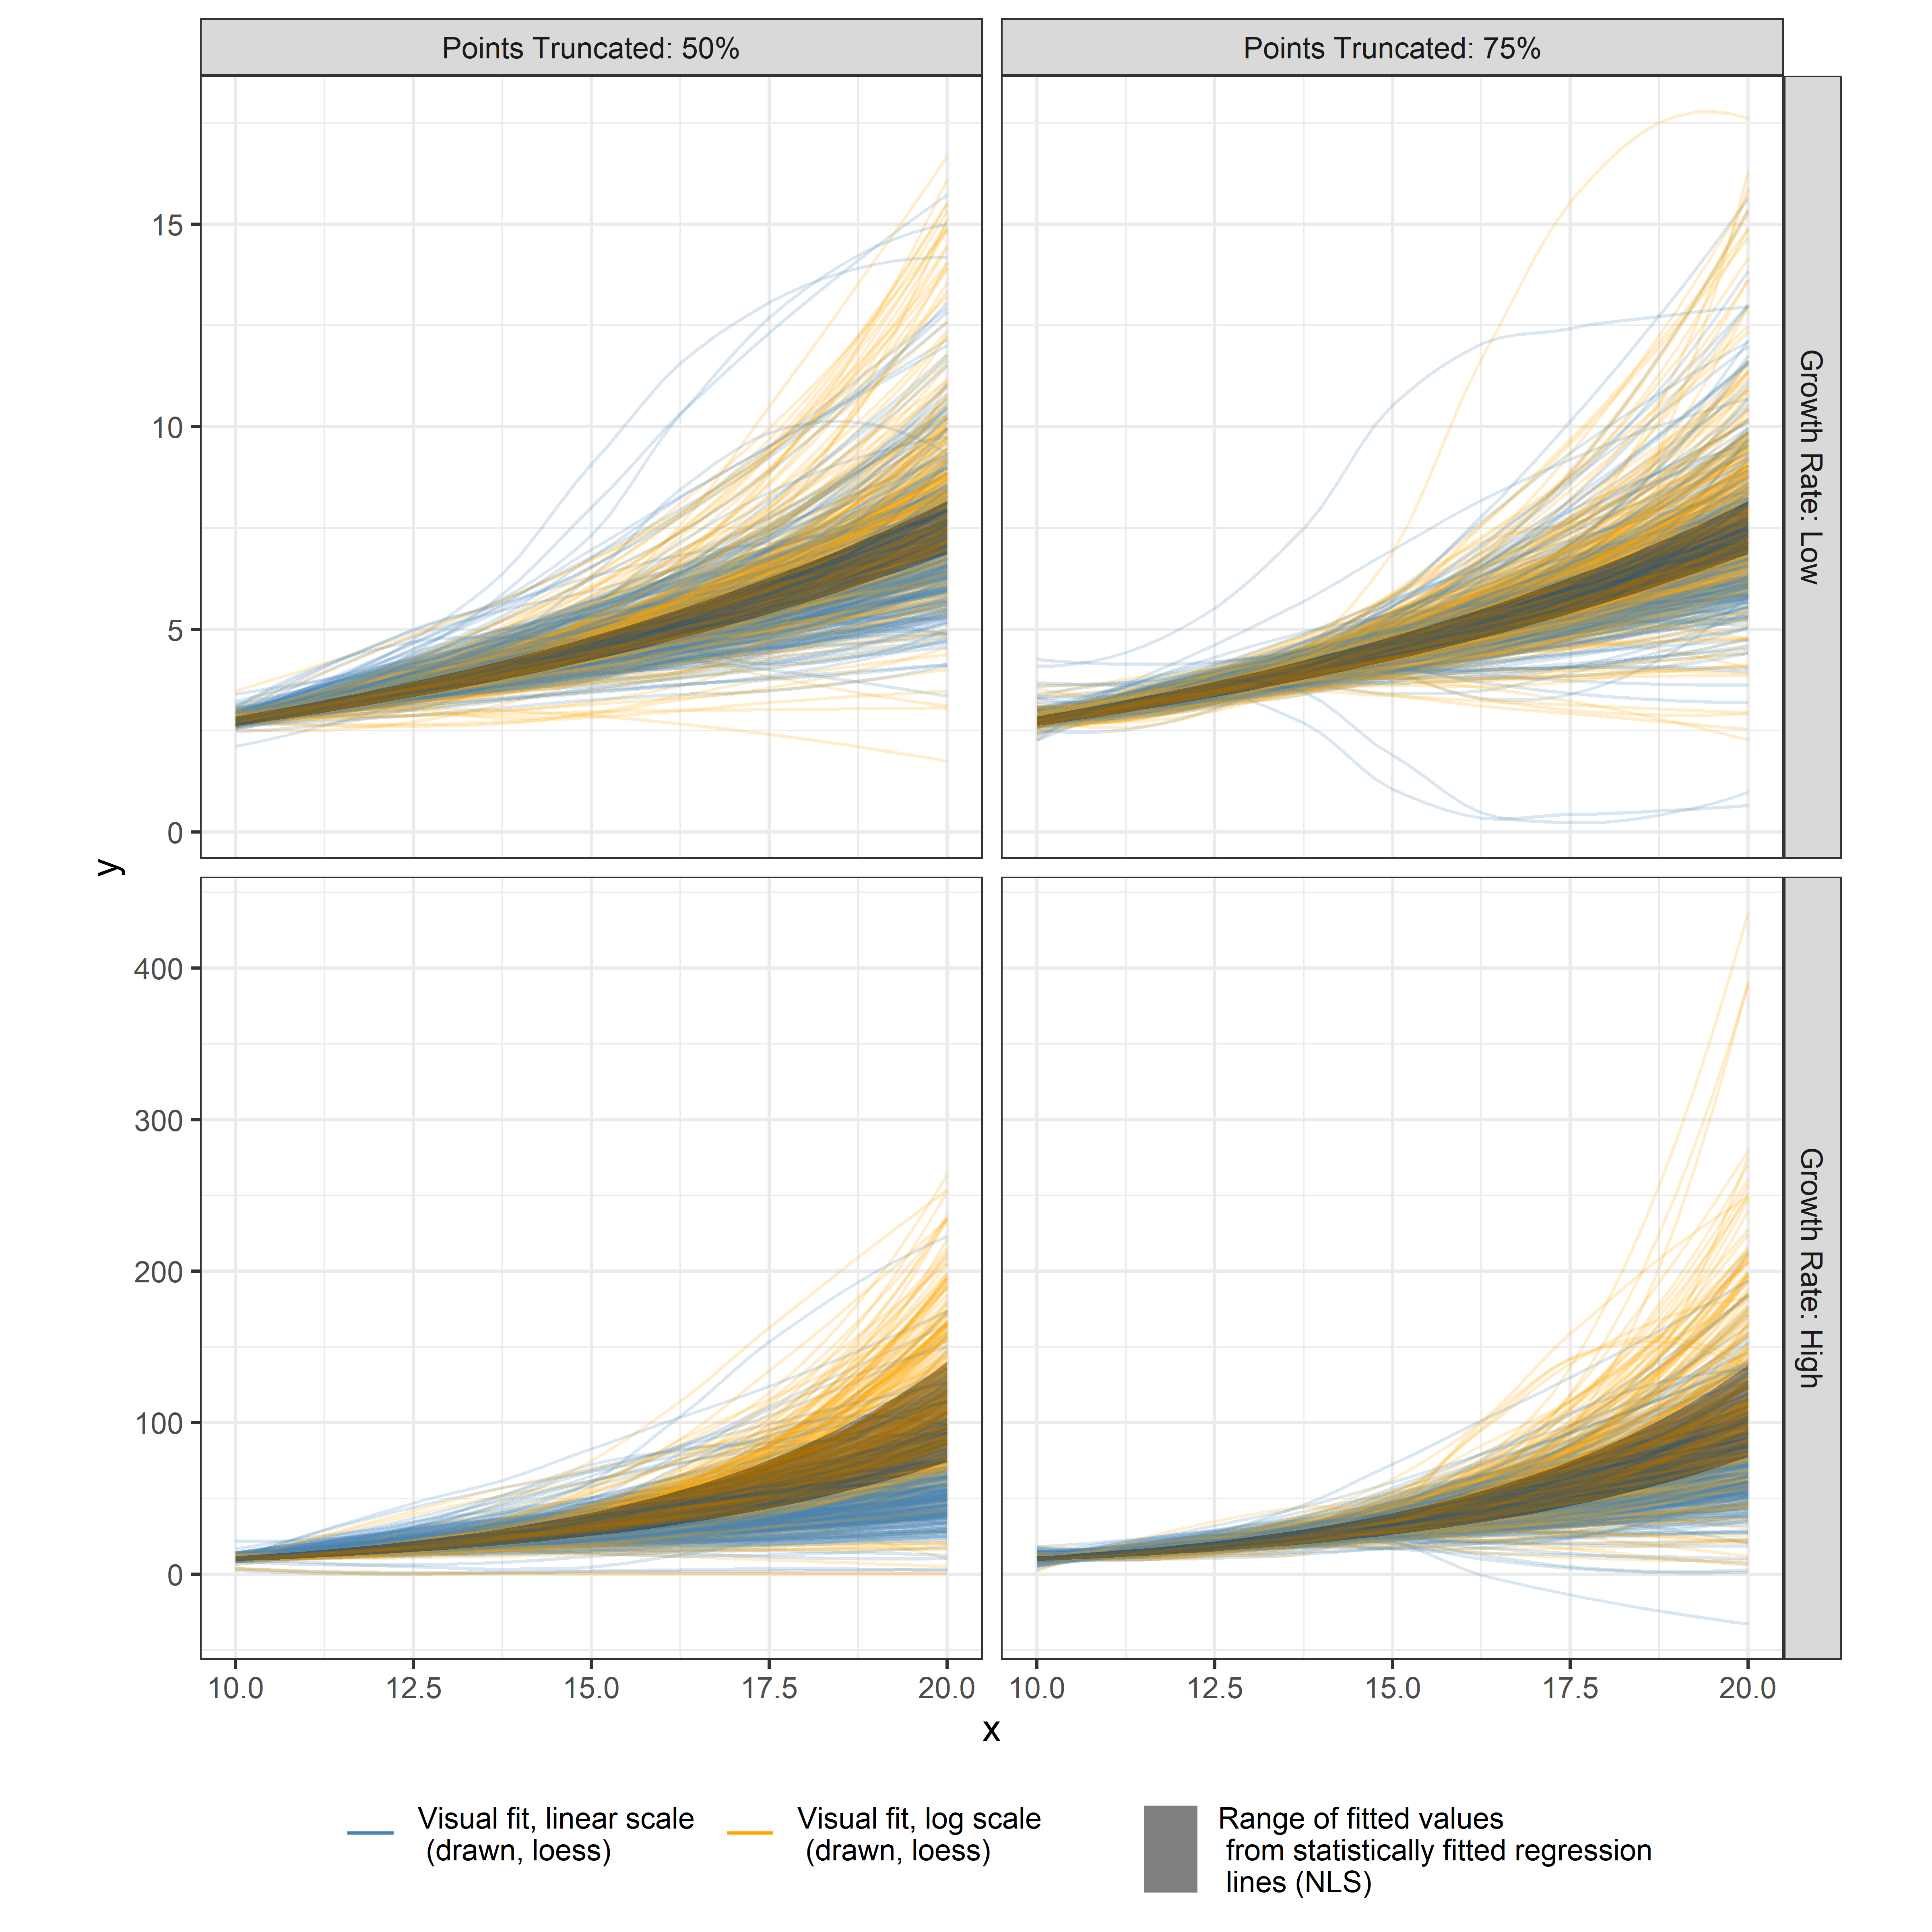
\includegraphics[width=\columnwidth]{images/exponential-yloess-spaghetti-plot-2-1}}
\caption{Spaghetti plot of results from a study which asked participants to forcast trends of exponentially increasing data. Participants drawn lines on the linear scale are shown in blue and the log scale are shown in orange. Variability in the statistically fitted regression lines occured due to a unique data set being simulated for each individual; the gray band shows the range fitted values from the statistically fitted regression lines.}
\label{exponential-yloess-spaghetti-plot-2-1}
\end{center}
\end{figure}

\section{Future Work}

In this work, we implemented and validated `You Draw It' as a new method
to measure the patterns we see in data. We demonstrated the use of
generalized additive models to statistically model participant feedback
data and generalized the analysis method to nonlinear trends. While
technical details of the development process are presented here, we
intend to create an R package designed for easy implementation of `You
Draw It' task plots in order to make this tool accessible to other
researchers. Further investigation is necessary to implement this method
with real data in order to facilitate scientific communication.

\bibliographystyle{sdss2020}
\bibliography{references.bib}
% \bibliography{references}

\end{document}

